\section{Fast Coresets in Practice}

We now provide an experimental analysis to verify that (1) Fast-Coresets obtain solutions of equal quality to sensitivity sampling while running significantly
faster, and (2) of the linear-time algorithms, only Fast-Coresets are guaranteed to satisfy the coreset property. We proceed by first
introducing our experimental setup, including the metrics, datasets, and algorithms being analyzed. We then follow this by a discussion of results regarding
both of the above claims.

\subsection{Experimental Setup}
\subsubsection{Metrics}
\label{sssec:metrics}

We analyze the coreset construction methods along two metrics -- coreset quality and construction time.  Although measuring runtime is standard, predicting coreset
quality is a more difficult task. Specifically, it is unclear how to confirm that a subset of points satisfies the coreset property over all solutions. To this
end, we use the following distortion measure
\[ \max \left( \dfrac{\cost(P, \calC_{\Omega})}{\cost(\Omega, \calC_{\Omega})}, \dfrac{\cost(\Omega, \calC_{\Omega})}{\cost(P, \calC_{\Omega})} \right),\]
where $\calC_{\Omega}$ is a candidate solution that was computed over the coreset~\cite{chrisESA}. This will be within
$1+\varepsilon$ if the coreset guarantee is satisfied but may be unbounded otherwise. 

We refer to this metric as the \emph{coreset distortion}. Naturally, values that are consistently close to $1$ suggest that solutions on the coreset are likely
viable on the full dataset.


\subsubsection{Algorithms}
\label{ssec:algorithms}

We compare our method (Algorithm~\ref{alg:main}) against 4 different benchmark coreset constructions:
\begin{itemize}
        \item \emph{Standard uniform sampling}. Uniform coresets are obtained by choosing a subset of $m \ll n$ points uniformly from $P$.
        \item \emph{Lightweight coresets \cite{bachem2018scalable}}. Lightweight coresets find the mean $\mu$ of the dataset and obtain per-point sensitivity estimates by $\hat{s}(p) = 1/|P| + \cost(p, \mu) / \cost(P, \mu)$. The goodness of this algorithm depends on how well these scores approximate \cref{eq:sensitivity}.
        \item \emph{Standard sensitivity sampling \cite{LS10}}. We follow the standard approach for sensitivity sampling outlined in Section~\ref{ssec:sens_sampling}.
        \item \emph{Welterweight coresets}: This is a generalized interpolation between lightweight coresets and the `heavy-duty' sensitivity sampling coresets. For any $j
            \in \{1,..., k\}$, we compute a coreset using sensitivity sampling with respect to a candidate $j$-means++ solution. For values $j \leq O(\log k)$,
            welterweight coresets share the runtime complexity of Fast-Coresets.
\end{itemize}

We take a moment here to motivate the welterweight coreset algorithm.  Consider that lightweight coresets are simply solving $1$-means to obtain sensitivity
values whereas sensitivity sampling is solving the $k$-means problem. Since the lightweight coreset has the advantage of being fast while sensitivity sampling
is more precise, one could hope to interpolate in order to get the best of the two worlds: computing an approximate $j$-means solution may allow to obtain
a more precise sampling distribution than that of lightweight-coresets, while being faster to compute than the $k$-means $O(1)$ approximation necessary for true
sensitivity sampling. We analyze the different choices of $j$ in Table~\ref{tbl:class-imbalance} and default to $j = \log k$ in the other experiments.

\subsubsection{Datasets}
\label{sssec:datasets}

We employ several real and artificial datasets to evaluate the quality of a coreset. 

For our real-world data, we utilize the Adult~\cite{Dua:2019}, MNIST~\cite{mnist}, Song~\cite{song}, Census~\cite{census}, and Cover Type~\cite{covtype}
datasets, whose characteristics are summarized in Table~\ref{tbl:datasets} below. These are standard datasets for coreset and clustering applications.

\begin{table}[htbp]
    \centering
    \begin{tabular}{lrr}
        Dataset & Points & Dim \\
        \hline
        \emph{Adult} & 48\,842 & 14 \\
        \emph{MNIST} & 60\,000 & 784 \\
        \emph{Song} & 515\,345 & 90 \\
        \emph{Cover Type} & 581\,012 & 54 \\
        \emph{Census} & 2\,458\,285 & 68 \\
        \hline
        \vspace*{0.1cm}
    \end{tabular}
    \caption{Description of real world datasets}
    \label{tbl:datasets}
\end{table}

\begin{table}[htbp]
    \centering
    \begin{tabular}{lrrrr}
        \hline
        Value of $r$ & 20 & 30 & 40 & 50 \\
        Runtime (s) & 13.5 & 14.3 & 15.7 & 16.1 \\
        \hline
        \vspace*{0.1cm}
    \end{tabular}
    \caption{Runtime in seconds of the \fkmeans algorithm as a function of $r$, as described in Section \ref{sssec:datasets}. Since $\log \Delta$ grows linearly
    with $r$, this evidences that \fkmeans has a linear time-dependency on $\log \Delta$.}
    \label{tbl:logdelta}
\end{table}

To complement those, we use several artificial datasets. Unless stated otherwise, $n = 50\,000$ and $d=50$.
\begin{itemize}

    \item \emph{$\log \Delta$ testbed}. Arrange $n - n'$ points uniformly in the $[-1, 1]^2$ square. Then, for $r \in \mathbb{Z}^+$, produce a sequence of
        points at $(0, 1), (0, 0.5), \cdots, (0, 0.5^r)$. Copy this sequence $n' / r$ times, each time with a different $x$ coordinate. The result is a dataset
        of $n$ points where the HST always has constant breadth but the branch depths (and correspondingly $\log \Delta$) grow linearly with $r$.
        This effect can be seen in table \ref{tbl:logdelta}.

    \item \emph{c-outlier}. Place $n-c$ points in a single location and $c$ points placed at a large distance away, for various constants $c$. 
	This data set constitutes an instance where we expect uniform sampling to perform poorly while all the other algorithms will do well.

    \item \emph{Gaussian mixture}. We seed $k$ multivariate Gaussians with varying cardinalities arranged randomly in high-dimensional space.  Each cluster has a center sampled from a multivariate normal with mean $0$ and variance $1\,000$ and each cluster is then i.i.d. samples multivariate normal distribution around
        this mean. Cluster sizes are defined as the random variable $|C_i| = \frac{n}{\kappa} \exp \left( \gamma(\rho_i - \frac{1}{2}) \right)$, where $\kappa$
        is the number of Gaussian clusters, $\rho_i$ is a uniform random variable, and $\gamma$ is a chosen hyperparameter\footnote{We show the effect of
        $\gamma$ on the cluster distribution in Figure~\ref{fig:effect-of-gamma} in the appendix.}. We obtain each cluster iteratively: once we have sampled one cluster of size
        $|C_0|$, we repeat the process for the next cluster with $|C_1| = \frac{n - |C_0|}{\kappa-1}\exp \left( \gamma(\rho_1 - \frac{1}{2}) \right)$.  Thus,
        each cluster has size $\frac{n}{k}$ when $\gamma = 0$ and the cluster sizes diverge as $\gamma$ grows. We default to $\gamma = 5$.
        
  This is a well-clusterable instance with respect to cost stability conditions, see \cite{AwS12,Cohen-AddadS17,KuK10,ORSS12}.

    \item \emph{Geometric}. Place $c k$ points at $(1, 0, 0, \cdots)$, $\frac{ck}{r}$ points at $(0, 1, 0, \cdots)$, $\frac{ck}{r^2}$ points
        at $(0, 0, 1, \cdots)$, and so on for $\log_r (ck)$ rounds. Thus, the data creates a high-dimensional simplex with uneven weights across the vertices. We
        default to $c = 100$ and $r=2$. 
	This data set constitutes an instance where we expect uniform sampling and lightweight as well as welterweight coresets to perform poorly while sensitivity sampling and \fkmeans are expected to perform well.

    \item \emph{Benchmark}. A specific distribution of points introduced in \cite{chrisESA} as a good testbed for coreset algorithms.  It has the property that
        all reasonable $k$-means solutions are of equal quality but are maximally far apart in the solution space. Thus, the dataset is fully determined by the
        number of centers $k$. We follow the advice in the benchmark's original presentation and produce three benchmark datasets of varying size before
        applying random offsets to each. We choose the sizes by $k_1 = \frac{k}{c_1}$, $k_2 = \frac{k - k_1}{c_2}$, and $k_3 = k - k_1 - k_2$ for $c_1, c_2 \in
        \mathbb{R}^+$.

\end{itemize}

In all real and artificial datasets, we add random uniform noise $\eta$ with $0 \leq \eta_i \leq 0.001$ in each dimension in order to make all points unique.
Unless specifically varying these parameters, we default all algorithms in~\ref{ssec:algorithms} to $k=100$ for the Adult, MNIST, and artificial datasets and
$k=500$ for the Song, Cover Type, and Census datasets. Our default coreset size is then $m = 40k$. We refer to the coreset size scalar as the \emph{$m$-scalar}.
We only run the dimension-reduction step on the MNIST dataset, as the remaining datasets already have sufficiently low dimensionality.

%\andrew{Add implementation details, machine specifics, etc.}

\subsection{Comparing Fast-Coresets to the State of the Art}
\label{ssec:alg_qualities}


\paragraph*{Comparison with standard sensitivity sampling.}

\begin{figure*}
\label{fig:coreset_size_on_sens_quality}
\centering
\begin{tabular}{lc}
    \rotatebox[origin=l]{90}{\bf \;\quad\quad\quad\quad\quad\quad\quad$k$-Median} &
    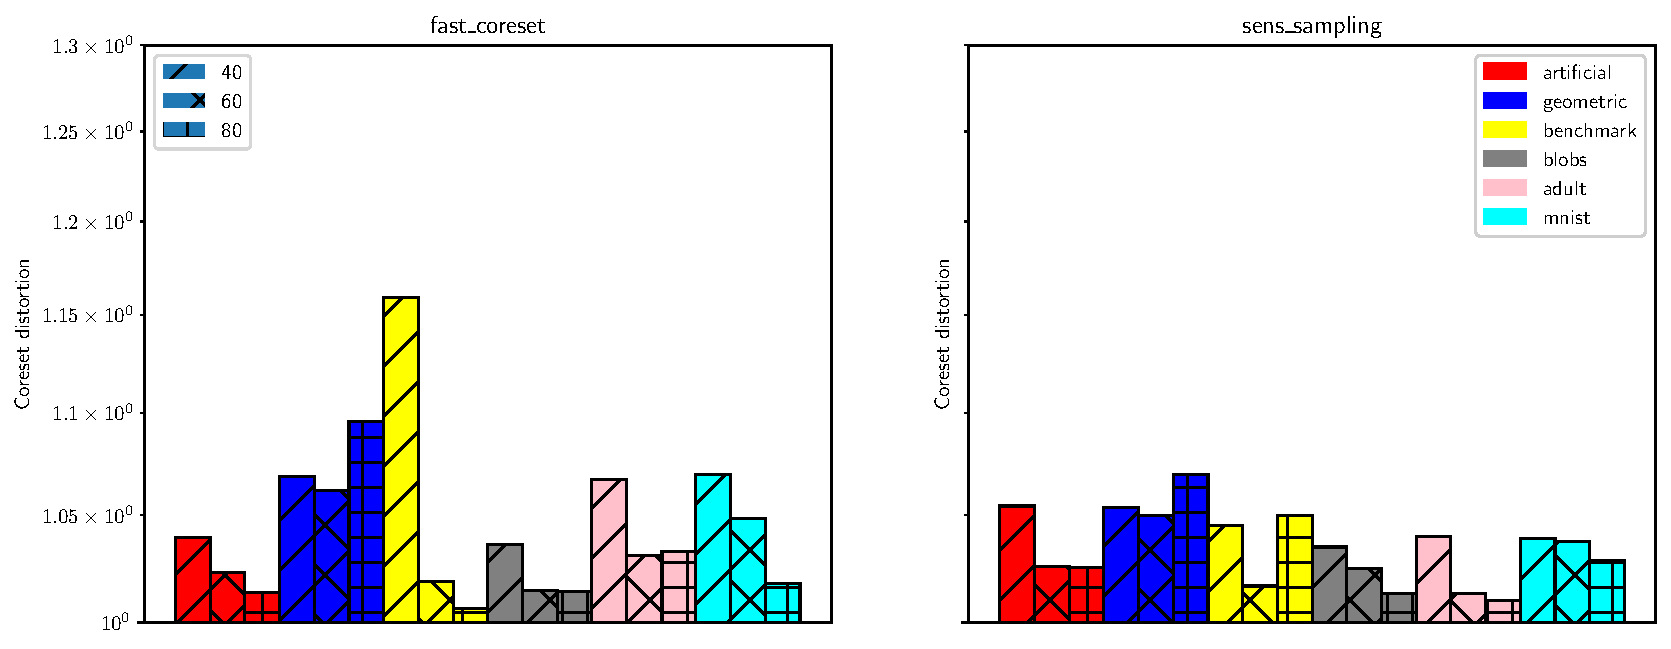
\includegraphics[width=.95\linewidth]{images/1/coreset_distortion-m_scalar_for_sens_sampling.pdf} \\

    \rotatebox[origin=l]{90}{\bf \;\;\quad\quad\quad\quad\quad\quad\quad$k$-Means} &
    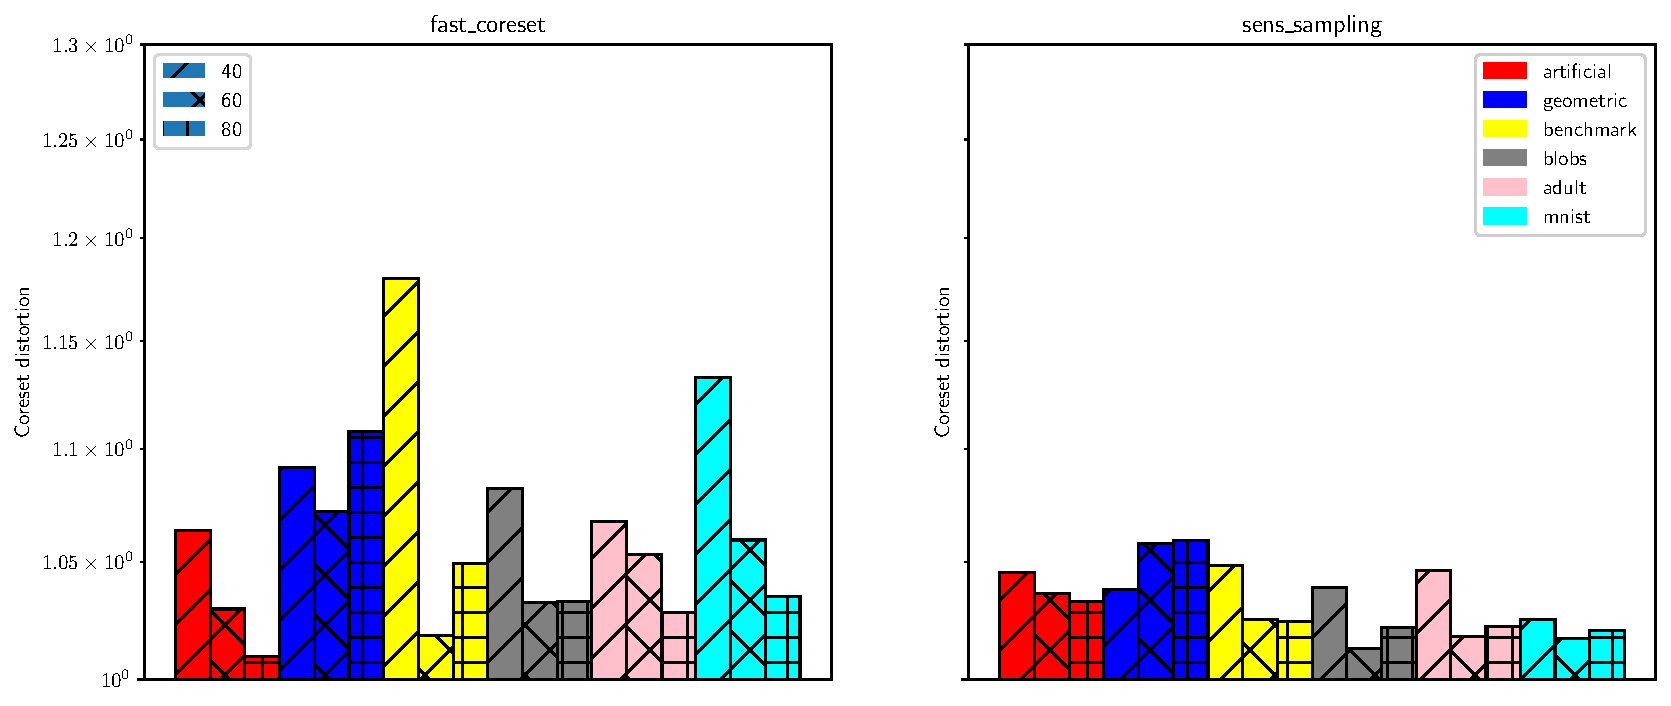
\includegraphics[width=.95\linewidth]{images/2/coreset_distortion-m_scalar_for_sens_sampling.pdf}
\end{tabular}
\caption{The effect of the coreset size on the distortion metric for sensitivity sampling approaches.
We point out that all distortion values are well below $\varepsilon = 0.2$.
Thus, for sufficient coreset sizes, there does not seem to be a meaningful difference between using Fast-Kmeans++ vs. regular Kmeans++.}
\end{figure*}


We first compare the Fast-Coreset algorithm with standard sensitivity sampling in terms of both quality and runtime.  To this end, the top of
Figure~\ref{fig:coreset_size_on_sens_quality} shows that, across datasets, the Fast-Coreset method produces coresets of consistent quality. Specifically, we
vary the $m$-scalar parameter and see that all distortion values are below $1.2$. Furthermore, choosing a sufficient coreset size ($m$-scalar$=80$) gives
distortion below $1.03$ for both Fast-Coresets and traditional sensitivity sampling. Despite this, we see in the bottom of
Figure~\ref{fig:coreset_size_on_sens_quality} that
varying $k$ from $50$ to $400$ causes a linear slowdown in sensitivity sampling but only a logarithmic one for the Fast-Coreset method.

This analysis confirms the theory predicted by \cref{thm:main}: Fast-Coresets run with little overhead while retaining the accuracy of sensitivity sampling.
Given this context, we did not add traditional sensitivity sampling to further experiments, as it is infeasible to run on large datasets.


\paragraph*{Comparison with other coreset methods.}

We now refer the reader to Figure~\ref{fig:coreset_size_on_quality}, where we show the effect of coreset size on our metrics across real datasets and methods by
sweeping over $m$-scalar values in $[20, 40, 60, 80]$. Despite the poor theoretical guarantees of uniform, lightweight, and welterweight coresets, we see that
they obtain competeitive distortions to sensitivity sampling while also running considerably faster in practice. We attribute this to the well-behaved nature of
the real-world datasets, where they have few outliers and classes of consistent sizes.

To evaluate this hypothesis, we apply the linear-time coreset algorithms on our artificial datasets in Table~\ref{tbl:artificial_failure}. These are constructed
to control for the characteristics of different data distributions and allow us to stress-test the coreset algorithms. For instance, the $c$-outlier dataset
tests whether a coreset algorithm is able to find all $c \ll n$ outliers. To this end, we see that, as expected, the uniform, lightweight and welterweight
algorithms all fail with a relatively high probability. Furthermore, we see a similar result in the Gaussian mixture and geometric datasets.

\begin{table*}[htbp]
    \centering
    \small
    \begin{tabular}{|c|cccc|cccc|cccc|cccc|}
        \hline
        & \multicolumn{16}{c|}{Method} \\
        \cline{2-17} & \multicolumn{4}{c|}{Uniform Sampling} & \multicolumn{4}{c|}{Lightweight} & \multicolumn{4}{c|}{Welterweight} & \multicolumn{4}{c|}{Fast Coreset} \\
        %\cline{2-17}
        % & \multicolumn{4}{c|}{Coreset Size} & \multicolumn{4}{c|}{Coreset Size} & \multicolumn{4}{c|}{Coreset Size} & \multicolumn{4}{c|}{Coreset Size} \\
        & $20k$ & $40k$ & $60k$ & $80k$ & $20k$ & $40k$ & $60k$ & $80k$ & $20k$ & $40k$ & $60k$ & $80k$ & $20k$ & $40k$ & $60k$ & $80k$ \\
        \cline{2-17}
        $c$-outlier & 710 & 126 & 488 & 89.4 & 1.09 & 1.04 & 34.3 & 1.02 & 1.09 & 1.04 & 21.8 & 34.3 & 1.12 & 1.05 & 1.03 & 1.02 \\
        Gaussian Mix. & 1.09 & 1.03 & 1.03 & 1.01 & 204 & 86.1 & 84.3 & 1.01 & 617 & 16.8 & 8.18 & 13.3 & 1.22 & 1.03 & 1.02 & 1.01 \\
        Geometric & 89.4 & 107 & 31.4 & 61.8 & 163 & 13.3 & 50.4 & 1.02 & 1.28 & 1.08 & 1.07 & 19.2 & 1.17 & 1.09 & 1.09 & 1.09 \\
        Benchmark & 1.09 & 1.04 & 1.04 & 1.03 & 1.14 & 1.05 & 1.05 & 1.03 & 1.12 & 1.05 & 1.06 & 1.04 & 1.54 & 1.35 & 1.14 & 1.02 \\
        \hline
    \end{tabular}
    \caption{Coreset distortions for each method on the artificial datasets. We report the results for coreset sizes $20k$-$80k$, with $k=100$ in all
    instances.}
    \label{tbl:artificial_failure}
\end{table*}

\begin{table}[htbp]
    \centering
    \begin{tabular}{lcccc}
        Algorithm & $\gamma = 0$ & $\gamma = 1$ & $\gamma = 3$ & $\gamma = 5$\\
        \hline
        LW Coreset & 1.03 & 1.03 & 1.36 & 2.17\\
        $j=2$ & 1.04 & 1.04 & 1.04 & 1.92\\
        $j=\log k$ & 1.04 & 1.04 & 1.04 & 1.95\\
        $j=\sqrt{k}$ & 1.05 & 1.06 & 1.04 & 1.18\\
        Fast Coreset & 1.03 & 1.03 & 1.04 & 1.12
    \end{tabular}
    \caption{The effect of $\gamma$ in the Gaussian mixture dataset on the coreset distortion. We report the means over 5 random dataset generations.
    Each generation had 50\,000 points in 50 dimensions, with 50 Gaussian clusters and coresets of size 4\,000. We set $k=100$.}
        \label{tbl:class-imbalance}
\end{table}

\begin{figure*}
\label{fig:lightweight_breaks}
\centering
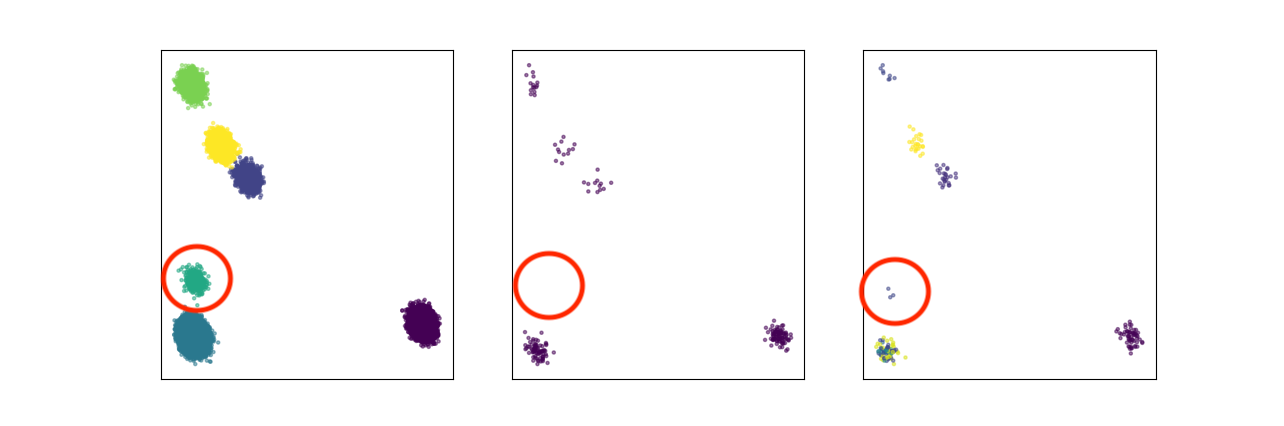
\includegraphics[width=.95\linewidth]{images/lightweight_breaks.png}
\caption{
The results of lightweight and fast-coreset constructions on a dataset of $n=100K$ points with clusters of varying size. Coresets have 200 points.
\emph{Left}: Original multivariate-Gaussian dataset. \emph{Middle}: Lightweight coresets fail to capture the cluster of $\sim$400 points.
\emph{Right}: The Fast-coreset construction runs in linear time but identifies all of the clusters.
}
\end{figure*}


Considering the failures of uniform, lightweight, and welterweight coresets on these three artificial datasets, we confirm that these methods
struggle with unevenly distributed cluster sizes. While it is clear why this occurs for uniform sampling, we take a moment to discuss the light- and
welterweight coreset constructions under this lens. Recall that lightweight coresets are sampling proportionate to the values
\[ s_{lw}(p) = \dfrac{\cost(p, \{\mu\})}{\cost(P, \{\mu\})} + \dfrac{1}{|P|},\]
where the first term is akin to importance sampling while the second is a uniform distribution. Since it is trivial to see that class imbalance breaks uniform
sampling, it remains to see how the cluster-sizes impact the $1$-means sensitivities. As a simple example, consider that a small cluster close to the mean
is unlikely to be sampled. 

This is evidenced in Table~\ref{tbl:class-imbalance}. There, we vary the Gaussian mixture dataset's
$\gamma$ parameter in order to study the effect that the class-distribution has on the coreset distortion. Since welterweight coresets are an interpolation
between the lightweight and sensitivity algorithms, we can consider this as ``How many centers do we need for $k$-means++ in order to handle class imbalance?''
Indeed, we find that lightweight coresets are the first to fail as cluster sizes diverge, followed by the $j=2$, $j=\log k$, and $j=\sqrt{k}$ welterweight
cases.

\begin{figure}
\centering
\begin{tabular}{lc}
    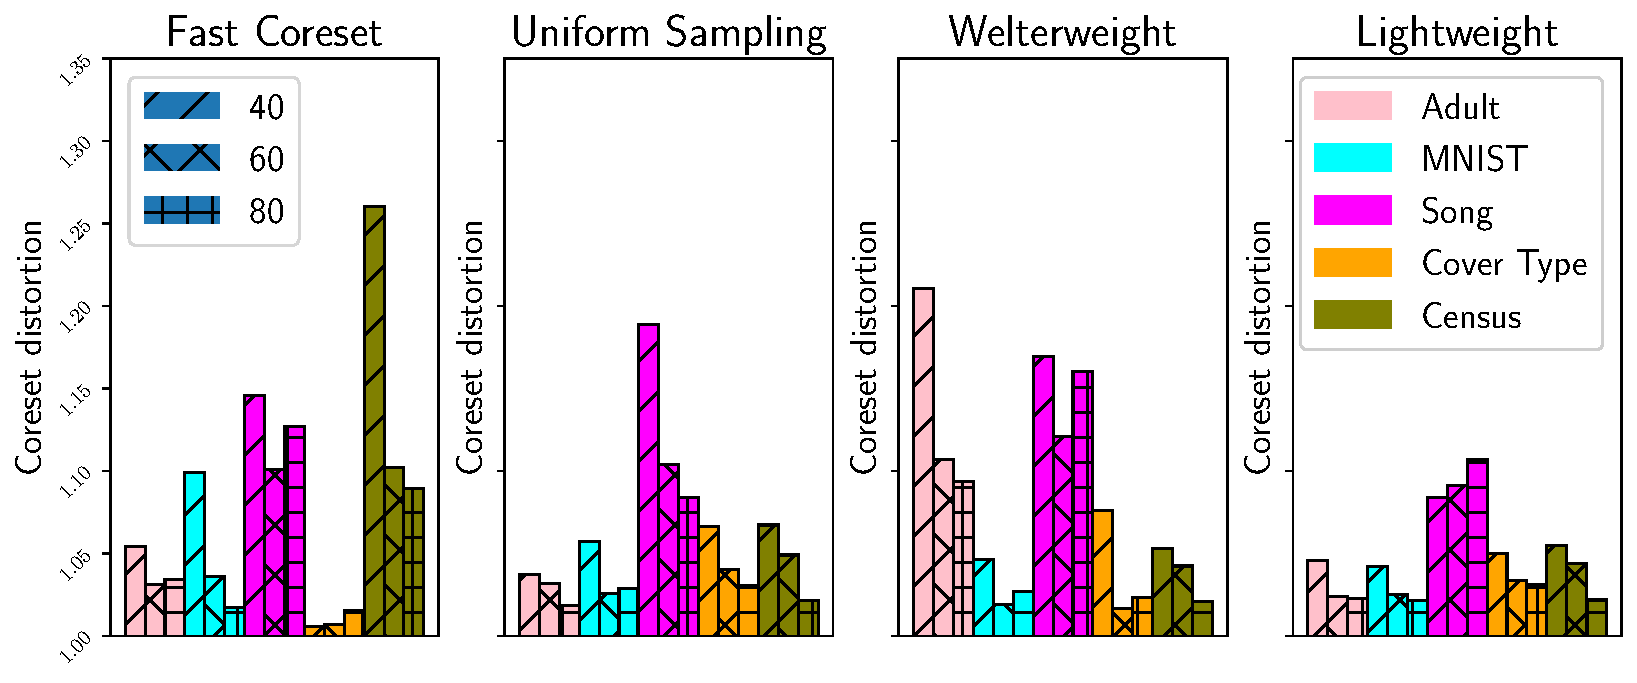
\includegraphics[width=\linewidth]{images/distortion_real_data} \\
    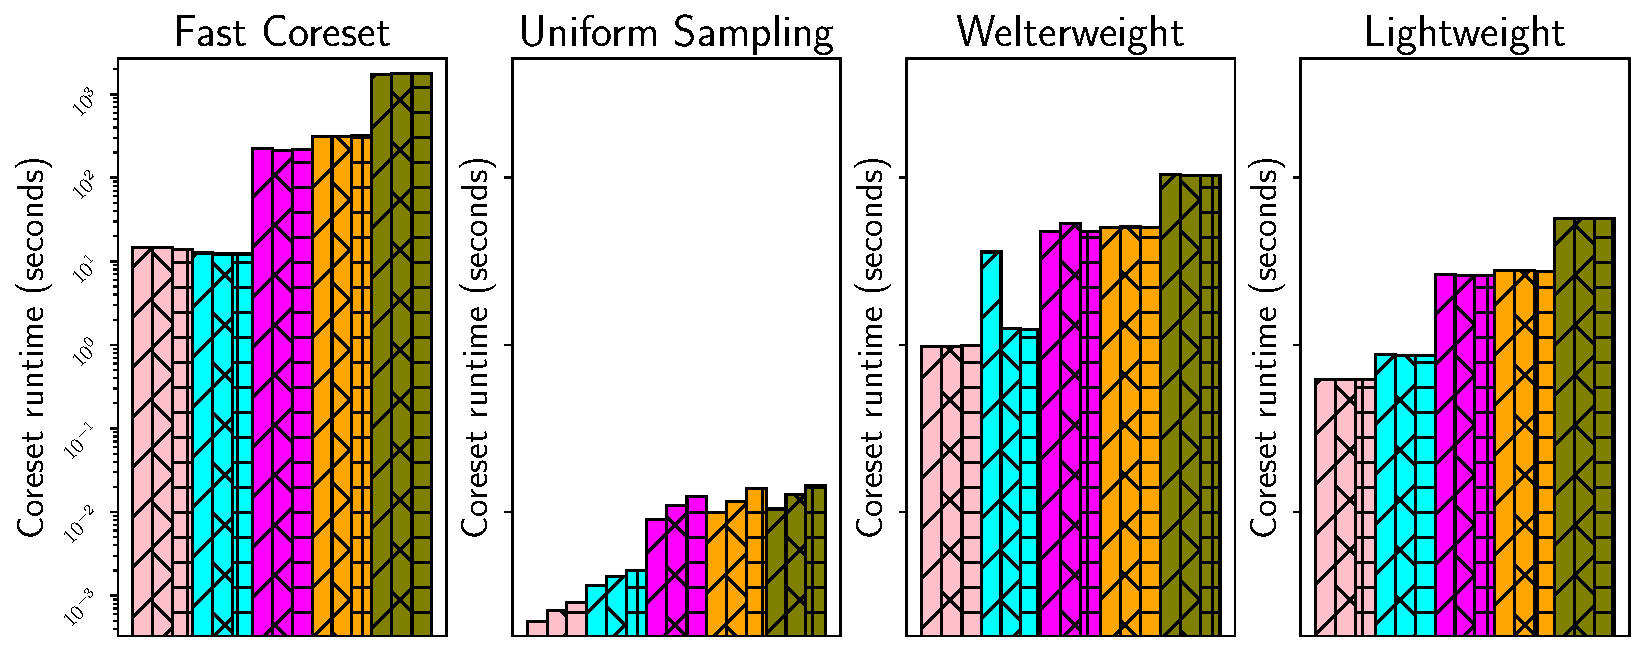
\includegraphics[width=\linewidth]{images/runtime_real_data}
\end{tabular}

\caption{\emph{Top}: The effect of the $m$-scalar on coreset distortion for real-world datasets. This is a visualization of the data in
Table~\ref{tbl:distortion}.  \emph{Bottom}: The effect of the $m$-scalar on the algorithm runtime for real-world datasets. All values are the mean over 5 runs.
The three bars represent samples of size $m=40k, 60k, 80k$.}

\label{fig:coreset_size_on_quality}
\end{figure}


\subsection{Conclusion}

The Fast Coreset method consistently outperforms sensitivity sampling with respect to runtime and is competitive with respect to coreset distortion.
Surprisingly to us, uniform sampling on real-world datasets always yields acceptable distortion results while being the fastest possible sampling algorithm. The
heuristic sensitivity approximations obtained from lightweight coresets and welterweight coresets to not significantly improve uniform sampling on real-world
datasets and do not offer a significant speedup compared to Fast-Coresets.  This suggests that uniform sampling is, at least empirically, the most efficient way
of summarizing datasets for downstream clustering tasks. However, uniform sampling has the major drawback that it has no guarantees and it is not possible to
determine from the sample whether it succeeded in summarizing the dataset to an acceptable degree. We identified cluster imbalance as the principal deciding
factor when uniform sampling fails. Verifying this apriori in sublinear time is hard.  Thus, as a fast, reliable summary with little overhead aside from reading
the data, we consider the Fast Coreset algorithm to be the best choice.

% \paragraph*{Additional evaluation on imbalanced clusters.}

% \david{Say what is the coreset size. Do you know why is Fast Coreset so bad as well? Would it be possible to increase it to have a good fast coreset?}
% \andrew{Are you asking why the fast coreset performs poorly in table~\ref{tbl:class-imbalance}? I think it does okay\ldots -- I can mention that this is for
% $m=20k$, which is a small coreset. I used a small one to emphasize the difference but can use a bigger one so that our scores aren't as bad.}
% \david{Ok, I didn't know the size was so small -- Yes, maybe a bigger one would be great (to be able to claim that fast coreset is consistently below 1.05 or something}

% As discussed, the sensitivities for lightweight coresets are obtained by a linear combination of a uniform distribution and each point's relative
% distance to the mean. Since the Gaussian mixture dataset has clusters of varying sizes, a small cluster that is close to the mean is unlikely
% to ever be sampled. We argue that, although this is a toy dataset, one can easily imagine real-world datasets that have this property. 
% As a simple solution, we see that the welterweight coreset obtains satisfactory solutions on the Gaussian mixture dataset for 
% \david{I don't know what you meant unfortunately}
% \andrew{I have not gotten to changing this paragraph, but it will basically say that the table of class imbalance shows that, as class imbalance grows, it is
% better to have $j>1$. I intend to add other values of $\gamma$ to that table.}

% A similar argument can be made for the more-challenging geometric dataset, where the cluster size decreases exponentially and all clusters are equidistant.
% We show furthermore that, for small values of $j$, sensitivities obtained according to
% solutions for $j$-means are insufficient to create a coreset for the geometric-progression dataset.
% 
% To further measure the effect that the class imbalance has on the quality of each coreset, we define a class imbalance parameter $\gamma$ and obtain each
% cluster's size by 
% 
% We see the effect of $\gamma$ on the coreset distortion in Table~\ref{tbl:class-imbalance}, where even
% small values of $\gamma$ can break the lightweight coreset construction.   Looking at the sensitivities computed via $j$-means++, we see that using $(j>1)$ is better at maintaining the coreset
% property for higher values of $\gamma$ but is still not guaranteed to obtain satisfactory compression. Despite this, sensitivity sampling consistently obtains
% coresets with low distortion.

% \david{the sentence "cluster sizes diverge exponentially as $\gamma$ grows linearly"
% is not super clear to me, because of the randomness. Also, since you are only showing two values of $\gamma$, it is hard to say that "it grows linearly": would
% it be possible to add the ratio max size / min size for $\gamma = 5$ ? This should be something close to $\exp(10)$ which is crazy huge compared to $50000$, so
% maybe not the right thing to plot...}
% \andrew{If I'm understanding correctly, you're saying that we should add a value for the largest cluster size divided by the smallest cluster size? I'm happy to
% do that. I think we could also just say what it is in expectation.}

